% !TEX encoding = UTF-8 Unicode
% !TEX TS-program = pdflatex
% !TEX spellcheck = en-US
% !TEX root = ../Report.tex

\chapter{System Compliance Analysis}

\subsection{MISRA C Analysys}

\subsection{Code Generation}
Inside this section, we are going to explain how we have generated the code for our control system. In particular we decided to generate only the source C code, because we didn't have in mind a specific architecture on which to implement our system, we leave the compilation to a future in which we have a target hardware. We decided to generate the code only for our control system and not for the entire Matlab project, because in we won't need to implement on a microcontroller the whole simulator, just the control system. 
\begin{figure} \label{Control Mask}
		\centering
		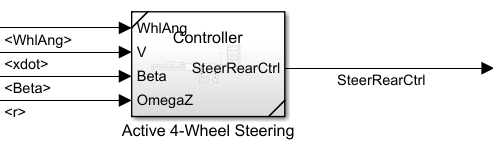
\includegraphics[width=0.7\textwidth]{Images/Simulator/ctrl-mask}
		\caption{Block Representation of the control system seen from outside}	
\end{figure}
As you can see from \ref{Control Mask} we will have the following inputs for our controller:
\begin{itemize}
\item $\delta_{w}$: Steering angle of the 4 wheels;
\item $\dot{x}$: Longitudinal speed of the vehicle;
\item $\beta_{u}$: Side slip angle;
\item $\omega_{z}$: Angular velocity.
\end{itemize}
And as output the objective of the controller, the control output:
\begin{itemize}
\item $\delta_{wr}$: Steering angle of rear wheels.
\end{itemize}
This block can therefore be interpreted, and will be translated into, a C function, with inputs as parameters of the function. This function/block also makes use of some parameters that describe the vehicle like mass, rotational inertia, cornering stiffness and also some characteristics of the environment that the vehicle is expected to operate in, like for example friction. You can anyway see all those values: parameters, input, outputs etc. in the code generation report that Matlab releases after the generation of the C code, as reported in \ref{Codegen Inports}. 
\begin{figure} \label{Codegen Inports}
		\centering
		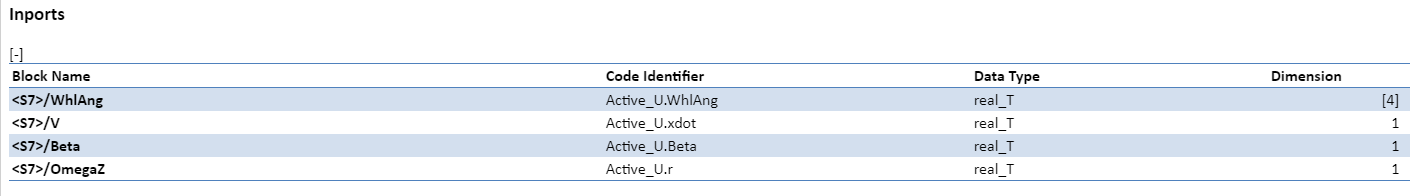
\includegraphics[width=0.9\textwidth]{Images/Simulator/codegen-inports}
		\caption{Input parameters of the C function obtained through code generation}	
\end{figure}
You will anyway be able to generate the report automatically using Simulink Coder directly from the Matlab project that is present on the shared Github repository. Because of our use of some functions that were available in the Simulink environment but not in the C code generation, we had to adapt our system to the new constraints, for example the first obstacle that we met during the design of the application was the impossibility of inserting the lqr algorithm for the optimal control inside a Simulink block and inside the generated C code, due to this limitation we were bound to have the output of the control algorithm in a tabled manner, we stored these results in a lookup table that the C function saves as a variable and uses directly, choosing one value or the other based on which is the most suitable for the actual state of the system, but completely unconscious of the lqr algorithm. Another weapon what we had at our disposal during the development with Simulink was the continuous logging of the signals, we could put a logger on each branch of the block scheme and it would record the evolution of that signal over time, this isn't possible with a C function and we had to abandon the logging, with the control leaving in a continuous present. It will be then work of the other part of the software, the simulator, the recording of the signals over time in the SIL tests. The generation of C Code was possible with many different targets, we decided for  a generic Real-Time target with a direction towards execution efficiency, instead of debugging purpose, because the math of the operations that are executed inside the controller is robust and all the interaction of the parts were already debugged in the Simulink phase.
\begin{figure} \label{Codegen Snippet}
		\centering
		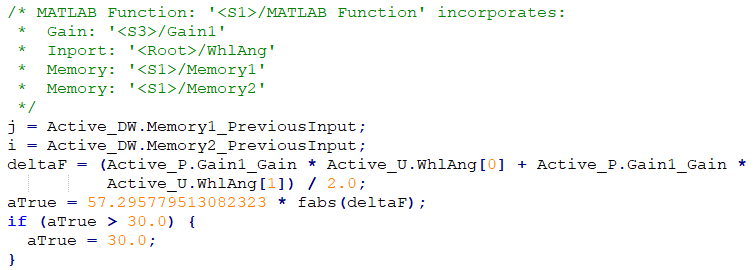
\includegraphics[width=0.7\textwidth]{Images/Simulator/codegen-snippet}
		\caption{Example of code obtained through automatic generation}	
\end{figure}
As you can see in figure \ref{Codegen Snippet} the automatically generated code is usually less readable than human written one, but it is logically correct and simplifies a lot the original block scheme, Simulink Coder is intelligent enough to eliminate or collapse together unnecessary or repeated blocks, thus creating a shorter and more on-point code.
